\documentclass[11pt,twoside]{article}

\usepackage{amsmath}
\usepackage{amssymb}
\usepackage{amsthm}
\usepackage{courier} % Required for the courier font
\usepackage{extramarks} % Required for headers and footers
\usepackage{fancyhdr} % Required for custom headers
\usepackage{graphicx} % Required to insert images
\usepackage{lastpage} % Required to determine the last page for the footer
\usepackage{listings} % Required for insertion of code
\usepackage{lipsum} % Used for inserting dummy 'Lorem ipsum' text into the template
\usepackage{mathtools}
\usepackage{subcaption}

\usepackage[margin=1in]{geometry}
\usepackage[usenames,dvipsnames]{color} % Required for custom colors

\begin{document}

\title{CSC411 - Project \#3}
\author{Yui Chit (Michael) Wong - 999806232\\Yijin (Catherine) Wang - 998350476}
\maketitle

\clearpage

\section*{Part 1}
\paragraph{Question}
Describe the datasets. You will be predicting whether the review is positive or negative from keywords that appear in the review. Is that feasible? Give 3 examples of specific keywords that may be useful, together with statistics on how often they appear in positive and negative reviews.

\paragraph{Answer}
It is feasible. The word "best" appears in 489 positive reviews and 365 negative reviews. The word "horrendous" appears in 3 positive reviews and 9 negative reviews. The word "awful" appears in 19 positive reviews and 103 negative reviews. Therefore, "best" could be useful to identify positive review, while "horrendous" and "awful" could be used to identify negative review.  (There are 1000 positive reviews and 1000 negative reviews in total.)

\clearpage

\section*{Part 2}

\paragraph{Question}
Implement the Naive Bayes algorithm for predicting whether the review is positive or negative. Tune the parameter $m$ using the validation set, and report how you did it and what was the result. Report the performance on the training and the test sets that you obtain. Note that compting products of many small numbers leads to underflow. Use the fact that $a_1a_2\cdots a_n = exp(loga_1 + loga_2 + \cdots loga_n)$. In your report, explain how you used that fact.

\paragraph{Answer}
In order to predict the review, we use the formula:
\[P(class | a_1, \cdots, a_n) = \frac{P(a_1, \cdots, a_n | class) P(class)}{P(a_1, \cdots, a_n)}\]
If $P(positive|a_1, \cdots, a_n) \geq P(negative|a_1, \cdots, a_n)$, we predict the review to be positive. Otherwise, we predict the review to be negative. Because $P(a_1, \cdots, a_n)$ is the same for $P(positive|a_1, \cdots, a_n)$ and $P(negative|a_1, \cdots, a_n)$, we only need to compare $P(a_1, \cdots, a_n | positive) P(positive)$ and\\ $P(a_1, \cdots, a_n | negative) P(negative)$.
\begin{align*}
P(a_1, \cdots, a_n | class) P(class) &= P(a_1|class) P(a_2|class)\cdots P(a_n|class)P(class)\\
&= exp(log(P(a_1|class))+\cdots+log(P(a_n|class))+log(P(class)))
\end{align*}
Based on the formula above, we only need to compare $log(P(a_1|positive))+\cdots+log(P(a_n|positive))+log(P(positive))$ and $log(P(a_1|negative))+\cdots+log(P(a_n|negative))+log(P(negative))$. Therefore, we implemented our part 2 python program based on the comparison.
\clearpage

\section*{Part 3}

\paragraph{Question}
List the 10 words that most strongly predict that the review is positive, and the 10 words that most strongly predict that the review is negative. State how you obtained those in terms of the the conditional probabilities used in the Naive Bayes algorithm.

\paragraph{Answer}
\begin{align*}
P(class | a_i) &= \frac{P(a_i | class) P(class)}{P(a_i)}\\
P(class | a_i) &= exp(log(P(a_i | class)) + log(P(class)) - log(P(a_i)))
\end{align*}
We use the formula above to compute and compare $P(positive | a_i)$ for all words in positive reviews and $P(negative | a_i)$ for all words in negative reviews.\\
The top 10 words that predicts positive are:\\
'ziembicki', 'unites', 'ulu', 'torrance', 'toiling', 'tiegs', 'swope', 'salability', 'rothchild', 'rollergirl'\\
The top 10 words that predicts negative are:\\
'zaltar', 'workout', 'unmercifully', 'szwarc', 'stuffing', 'slunk', 'salkinds', 'refugees', 'popeye', 'omegahedron'\\
Although most of the words does not make sense intuitively to make strong prediction, they showed up in the result because they only appeared in one class. For example, 'ziembicki' is only in positive reviews, 'popeye' is only in negative reviews.
\clearpage

\section*{Part 4}
\paragraph{Question}
Train a Logistic Regression model on the same dataset. For a single movie review, For a single review $r$ the input to the Logistic Regression model will be a $k$-dimensional vector $v$ , where $v[k]=1$ if the $k$-th keyword appears in the review $r$. The set of keywords consists of all the words that appear in all the reviews.

Plot the learning curves (performance vs. iteration) of the Logistic Regression model. Describe how you selected the regularization parameter (and describe the experiments you used to select it).

\paragraph{Answer}
When working on this part of the project, we first obtained the whole list of keywords from the training set (both positive and negative reviews). Then for each review in the testing and validation set, we will create a $k$-dimensional vector $v$, where $v[k]=1$ if the $k$-th keyword appears in the review. If a review from the test or validation set contains a keyword that isn't in the training keyword set, it would be ignored. We then stack the vectors together to get a `$x$' for each of the training, test, and validation. 

We then used the $x\_train$ to train the model and test the performance on $x\_test, x\_val$. We used tensorflow to implement the architecture of the model. We used one-hot encoding for the output. For the network model, we only have 1 input layer and an output layer that has sigmoid activiation function. We also have a $L2$ penalty for the weight (used as regularization). The training step is done by the Adam Optimizer, which is a variant of gradient descend. Also, each iteration we will take a randomly chosen mini batch from the original training set to speed the process and avoid running into local minima.

When picking the parameter, it's done mostly by trial and error. We tested different values for the parameters, and selected the best one based on the performance on validation.

I ran the training step for 10000 iterations, and the final performance on training set and test set are 100\% and 86\% respectively. The result of the training vs. iteration is summarized below:

\begin{figure*}[h]
	\centering
	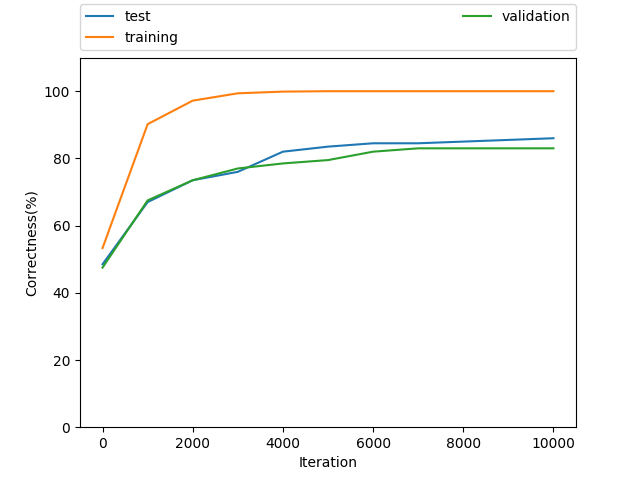
\includegraphics[scale=0.8]{part4.png}
	\caption*{Learning curve}
\end{figure*}

\clearpage

\section*{Part 5}
\paragraph{Question}
At test time, both Logistic Regression and Naive Bayes can be formulated as computing

\[\theta_0+\theta_1I_1(x)+\theta_2I_2(x)+\cdots+\theta_kI_k(x) > thr\]

in order to decide whether to classify $x$ as 1 or 0 . Explain, in each case, what the $\theta$‘s and the $I$‘s are.

\paragraph{Answer}
Assume $x$ is one review which is a $k$-dimensional vector where $k$ is the total number of unique words in the set.\\
$\theta_0 = log(P(positive)) - log(P(negative))$.\\
$I_i(x)$ is the $i$th word of input $x$. $I_i(x)$ is either 1 or 0, where 1 means that $i$th word is in review $x$, 0 means that $i$th word is not in review $x$.\\
$\theta_i = log(P(word_i | positive))  - log(P(word_i | negative))$
\clearpage

\section*{Part 6}
\paragraph{Question}
Compare the top 100 $\theta$s that you obtained using Naive Bayes and Logistic Regression.
\paragraph{Answer}
The average of $\theta$ from Naive Bayes is 0.176375, with standard deviation 0.125596.\\
The average of $\theta$ from logistic regression is 0.004004, with standard deviation 0.001090.\\

By comparing the top 100 $\theta$s with corresponding words from Naive Bayes and Logistic Regression, we found that:\\

Common positive words are:\\
{'hilarious', 'outstanding', 'terrific', 'change', 'memorable'}\\

Common negative words are:\\
{'bad', 'waste', 'stupid', 'nothing', 'boring'}\\

Number of positive words from Naive Bayes = 59\\
Number of positive words from Logistic Regression = 40\\
Number of negative words from Naive Bayes = 41\\
Number of negative words from Logistic Regression = 60\\

Although not many words are in common, it is clear to see that most of the words do strongly predicts positive or negative.
\clearpage

\section*{Part 7}
\paragraph{Question}
We are supplying you with word2vec embeddings for a list of word. Show that the word2vec embeddings work for figuring out whether $t$ appears together with $w$ or not using Logistic Regression. Describe the experiment you performed and its results.

\paragraph{Answer}
When working on this part of the assignment, we first need to set up the $x$'s of the each of training, test, and validation set. Since in this part of the assignment, we are just trying to determine if we can predict if words would occur together, a review being positive or negative does not matter too much. Thus we decided to just take files from the $pos$ review within each dataset.

When setting up the x for each dataset, we will first randomly choose multiple files within the dataset (because looping through all files would take too long). Then for each file, we will create a list of lower case words that has the punctuation removed. Then we will loop through that list, and for each pair of neighbouring words, we will find the corresponding embedding, concatenate it, and stack it into $x$. Note that if the any of the words doesn't have a corresponding embedding, it would be ignored. We will label this as $[1, 0]$ to indicates the words are neighbouring, and vstack it to the y.

When looping through the list of words in all the randomly chosen files within the dataset, we will keep track of the set of unique keywords. We will also keep track of the set of unique pairs of words that we added into $x$. After looping all the randomly selected files, we will have to create sample $x$'s where the two words in $x$ is not neighbouring. To do this, we will randomly pick two word from the unique keyword set, make sure they are not neighbouring (by checking the list of pair words), find the corrsponding embedding, and add the concatenation into $x$. We will label this as $[0, 1]$ to indicate the words are not neighbouring, and vstack it to y.

After obtaining $x\_train, x\_test,$ and $x\_val$, we will pass them into a tensorflow model with the following architecture:
\begin {itemize}
	\item Input layer has size $256$ (concatenation of 2 vectors with size 128).
	\item Output layer that has two outputs (the two classifiers). Each outputs if fully connected with the layer below. The activation function is sigmoid.
	\item The weight that connects input to output layer is randomly generated.
	\item We placed a softmax on top the output layer, and we use the negative log loss function as our cost function.
	\item We added a L2 regularization.
	\item When training, we will use a mini-batch. We also use the Adam Optimizer for each training step, which is a variant of gradient descent.
\end {itemize}

There are multiple parameters when it comes to the model aboved: $\alpha, \lambda$, mini-batch size etc. As usual, they are chosen based on the best validation results through trial and error. As for how many files we are randomly picking when setting up the $x$'s, we want to pick a number that gives a big enough data within the dataset while making sure the runtime does not take too long.

The final performance on training, validation, and test sets are 75\%, 70\%, and 70\% accordingly after 15000 iterations of gradient descent. The learning graph is shown as below:

\begin{figure*}[h]
	\centering
	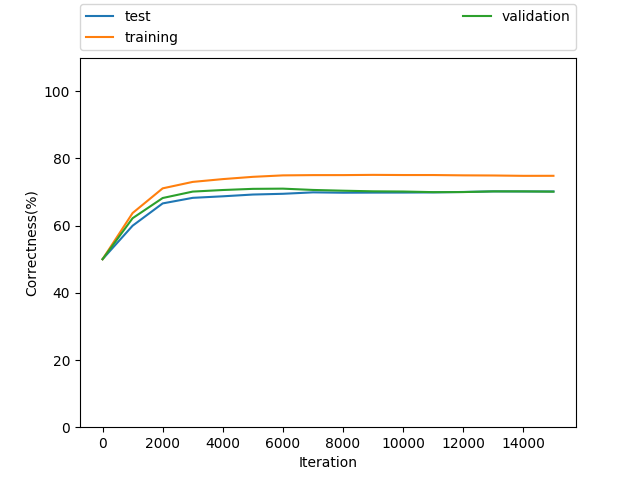
\includegraphics[scale=0.8]{part7.png}
	\caption*{Learning curve}
\end{figure*}

\clearpage

\section*{Part 8}
\paragraph{Question}
The reason word2vec works is that words that appear in similar contexts have similar embeddings (in the sense that the Cosine or Euclidean distance between the embeddings is small). Investigate this by finding the 10 words whose embeddings are closest to the embedding of “story”, and the the 10 words whose embeddings are closest to the embedding of “good.” Find two more interesting examples like that that demonstrate that word2vec works.

\paragraph{Answer}
The similar words of 'story' we found using either euclidean distance or cosine distance are:\\
'plot', 'film', 'benito', 'simmer', 'sitter', 'lift', 'domineering', 'ricci', 'interviews', 'acclaim'\\
The similar words of 'good' we found using either euclidean distance or cosine distance are:\\
'bad', 'great', 'wonderful', 'reinforcing', 'decent', 'funny', 'manipulate', 'underused', 'admiral', 'perplexing'\\
The other interesting examples we get are:\\
"teacher" + "student" = "expects"\\
"war" + "man" = "divesting"\\
(Note: we found the resulting word after operation by the embedding vector with closest cosine distance but not one of the words used for calculation)
\clearpage


\end{document}